\section{Introduction}
% \subsection{X-ray fluorescence data acquisition method}
\subsection{Motivation}
The work presented is built upon contributions made by dr. inż. Bartłomiej Łach in his doctoral thesis entitled \emph{Rozwój systemu detekcyjnego do obrazowania przestrzennego rozkładu pierwiastków metodą fluorescencji rentgenowskiej}\cite{Lach2022}  (eng. \emph{Development of a detection system for spatial imaging of element distribution using X-ray fluorescence}).

His dissertation was dedicated to development of system for non-invasive analysis of works of art that uses X-ray radiation to carry out measurements. 
The system presented was designed to provide a map of element distribution in the top layers of the object, offering essential information for analyzing the pigments used in the artwork. 
The results provided by analysis could be source of important knowledge for conservators of monuments and art, informing them about the object's state of preservation, quality of past maintenance processes, the work's authenticity and leading to the expansion of previous state of knowledge.

The most popular technique to perform measurements, namely MA-XRF (Macro X-Ray Fluorescence), operate by scanning selected parts of art point by point. 
This method is characterized by high spatial and energetic resolution. 
However, due to usage of polycapillary lenses it is limited to performing scans on 2D surfaces.
Another drawback this method shows is long measurement time. 
For example, scanning a painting with an area of $65 \times 45$ $\text{cm}^{2}$, a resolution of $1300 \times 900$ pixels, and a  dwell time of $10$ ms per pixel could take about $3.5$ hours.\cite{Alfeld2013}. 

An alternative method involves scanning not just a single point but multiple points within a specified area of the surface, by utilizing FF-XRF (Full-Field X-Ray Fluorescence). 
This exact approach was implemented by researchers at AGH University of Krakow in the DETART (Detector for Art) data acquisition system. 
DETART not only can scan large portion of the surface (over $10^5$ pixels at the same time), but it is also capable of performing scans of 3D objects without losing spatial resolution thanks to near infinite depth of field provided by pinhole camera. 

After data acquisition part, the analysis can be performed. 
Łach proposed three different methods for analyzing data: ``standard'' ROI (Region Of Interest) method and two different machine learning algorithms: PCA (Principal Components Analysis) and NFM (Non-negative Matrix Factorization). 
Each of them had its advantages and disadvantages. 
In the end, there may not be a single method that is universally superior. 
However, employing multiple methods allows us to draw more comprehensive conclusions, leveraging the strengths of each and compensating for their respective limitations.

\subsection{Concept}
Concept of this thesis is heavily inspired by the work presented in \cite{Jones2022}. 
The authors of this article introduced the idea of a CNN (Convolutional Neural Network) model tasked with classifying every sample measured with XRF as one pigment class. 
They trained the model on synthetic data first, achieving through it an accuracy of 55\% after performing tests on real XRF spectra, and 96\% after applying transfer learning using small quantity of real XRF samples.  
This approach is pretty convenient for further usage thanks to full automation of the process. 
It also presents high accuracy after application of transfer learning.
However, there are some downsides to consider:
\begin{itemize}
    \item The model can only classify pigments it has learned about
    \item It does not provide any information about signals coming from elements, which may offer some valuable insights about the studied object
\end{itemize}
A potential solution to these problems may be to shift the focus from classifying pigments to classifying elements. A multi-label classification approach might be used to assess existence of each learned element independently from the tested pigment. This approach is more similar to algorithms used in Łach's thesis.

\subsection{Introduction to XRF}
\subsubsection{Physics fundations}
XRF method utilizes X-ray radiation to provide data for further analysis of objects exposed to radiation. 
It is considered harmless when used in small doses and low intensity.  
Therefore, it can be used to study delicate objects, such as art, monuments, geological and biological samples.
Characteristic X-ray fluorescence radiation is type of secondary radiation generated in matter under the influence of radiation from an external source - X-ray tube in research setting.

The fundamental physics behind the whole process is the phenomenon of photoelectric absorption.
In this process, one of photons transfers all its energy to one of the electrons bound to the inner electron shell of an atom. 
Consequently the electron is ``knocked out'' from its position on the shell, leaving a vacant space (hole) in the shell. 
Absorption can only occur if the energetic criterion is satisfied; that is, the energy that photon gives to the electron must be greater than the binding energy of electron in the specific shell.

After the emission of the electron, the state of the atom is unstable (excited), which results in electron jumping from a higher level to the vacancy left by the emitted electron, creating its own vacancy.
The entire process continues until the atom reaches an equilibrium state.

Electrons placed on outer shells have higher energy than electrons on lower shells. 
According to the law of conservation of energy, something must happen to the excess energy - the emission in the form of characteristic photon occurs. 
The binding energies on each shell are unique features of every element and are related to the energies of characteristic photons.
These energies are also known as spectral lines, e.g. when electron jumps from shell L to K it releases energy equals to difference between their binding energies: K$_\alpha$ spectral line, from shell M to K - K$_\beta$ spectral line, and so on.
Therefore, with \emph{a priori} knowledge about energies of specific spectral lines, one should be able to identify elements present in measured spectrum - see \prettyref{fig:photons_energy}.

\begin{figure}[h] 
  \centering     
  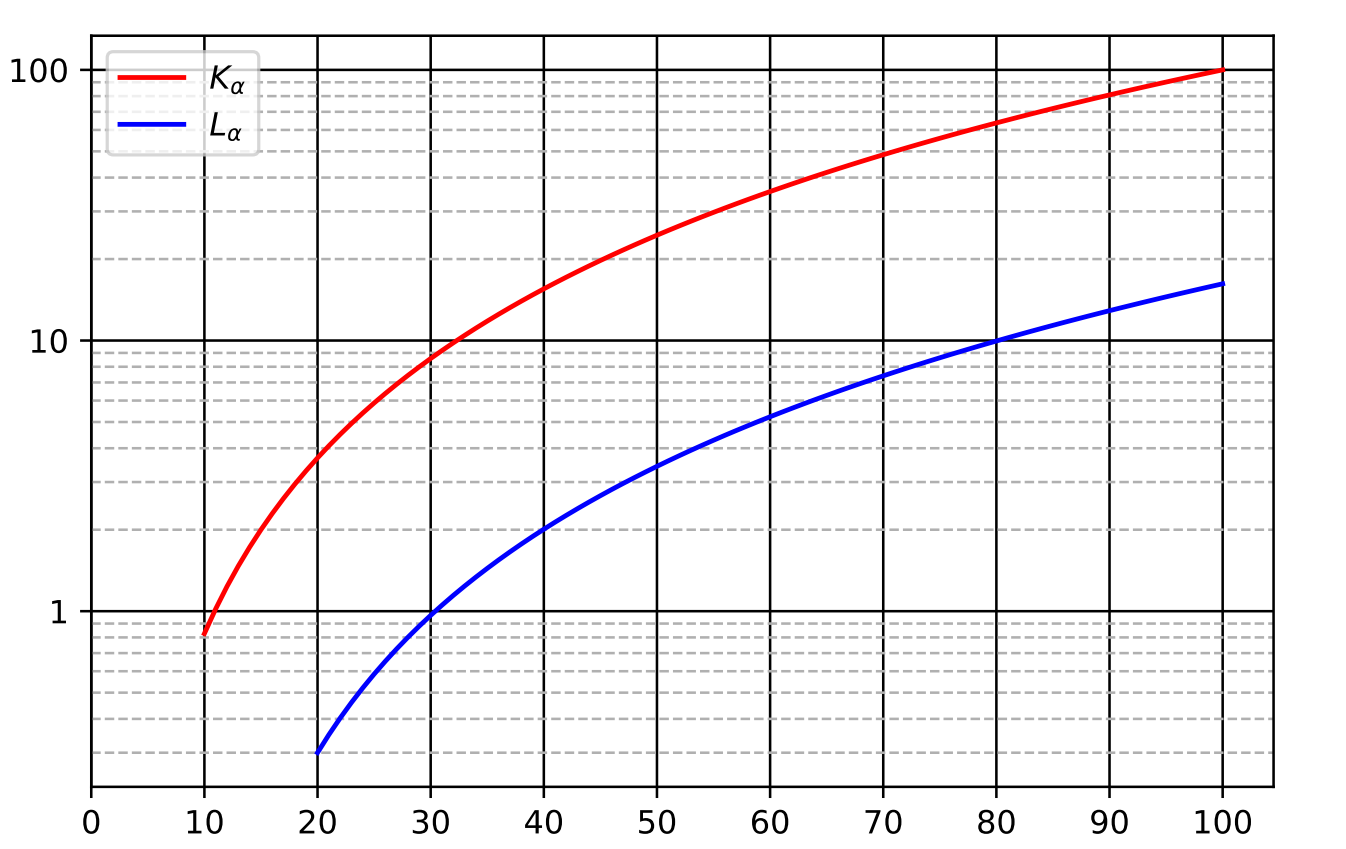
\includegraphics[width=0.8\textwidth]{img/dependence_of_photons_energy.png} 
  \caption{The dependence of the energy [KeV] of photons  emitted due to transitions of electrons from the L to K level (K$_\alpha$ spectral line) and M to L level (L$_\alpha$ spectral line) as a function of the atomic number Z [-]. Source: \cite{Lach2022}}
  \label{fig:photons_energy}
\end{figure}

At the same time competitive process can occur - Auger electron ejection. This process involves the following events\cite{augerElectron}:
\begin{enumerate}
    \item An electron on the inner shell is ejected by a photon, creating a vacancy.
    \item A secondary electron drops down to fill the vacancy.
    \item If sufficient energy is emitted, a tertiary electron is ejected (Auger electron)
\end{enumerate}
